
\chapter{Changes in 0.8.1}
\label{ch:081changes}


%%%%%%%%%%%%%%%%%%%%%%%%%%%%%%%%%%%%%%%%%%%%%%%%%%%%%%%%%%%%%%%%
\section{Support for setting and output files}
\label{sec:filesSupport}

\subsection{Software specific settings}

The element \xelem{SoftwareSettings} has been added to common 
task types (estimation and simulation) description allowing for optional storage of software 
specific settings -- in agreement with recent MDL task proposal. 
Note that optimal design tasks can use this option already since version 0.7.2, \cite{Swat:2015b}. 


\subsection{Output files}
This new element \xelem{OutputFile} offers the specification of the 
\begin{itemize}
\item 
target SO file
\item 
or a target-specific results files
\end{itemize}
as the example code below shows
\lstset{language=XML}
\begin{lstlisting}
    <ModellingSteps xmlns="http://www.pharmml.org/pharmml/0.8/ModellingSteps">
        
        <TargetTool oid="targetTool">
            <TargetToolName>PFIM</TargetToolName>
        </TargetTool>

        <!-- Standard Output file -->
        <OutputFile oid="resultsSO">
                <ds:path>task_XYZ_SO.xml</ds:path>
        </OutputFile>

        <!-- or alternatively any number of output files -->
        <OutputFile oid="res1">
                <ds:path>results1.csv</ds:path>
        </OutputFile>

        <OutputFile oid="res2">
                <ds:path>results2.csv</ds:path>
        </OutputFile>
        <!-- ... -->        
\end{lstlisting}
Note, that only the \xelem{path} is mandatory, \xelem{format} and \xelem{delimiter}
are optional.

%%%%%%%%%%%%%%%%%%%%%%%%%%%%%%%%%%%%%%%%%%%%%%%%%%%%%%%%%%%%%%%%
\section{Optimal design extensions}
\label{sec:OEDextentions}

Optimal design (OD) and related task has been extended with few missing components.

\subsection{Parameter settings}
The element \xelem{ParametersToEstimate} has been added to the optimal design task description -- 
an element featured in estimation task already. Its reuse here allows for specification 
of parameters initial values, lower/upper bound values assignment or indication of which 
parameters are to be kept fixed.


\subsection{\emph{Stage} definition}
Although described in the optimal design specification, \cite{Commets2015}, 
we have managed to ignore it when implementing the OD support in PharmML v0.7.2,
\cite{Swat:2015b}, which are now fully supported. 

The following examples are borrowed from the OD example collection 
\cite{CommetsExamples2015} and visualise the options available for the new 
\xelem{StageDefinition} element
\begin{itemize}
\item 
Single stage specification
\lstset{language=MLX}
\begin{lstlisting}
        DS{name=t1, element=doseTime, range=[0,6], stage = 1 }
\end{lstlisting}
with PharmML implementation
\lstset{language=XML}
\begin{lstlisting}
        <StageDefinition>
            <math:LogicBinop op="eq">
                <math:Stage/>
                <ct:Real>1</ct:Real>
            </math:LogicBinop>
        </StageDefinition>
\end{lstlisting}
\item 
Stage set specification
\lstset{language=MLX}
\begin{lstlisting}
        DS{name=t1, element=doseTime, range=[0,8], stage = {1,2,3} }
\end{lstlisting}
\lstset{language=XML}
with PharmML implementation
\begin{lstlisting}
        <StageDefinition>
            <math:LogicBinop op="eq">
                <design:Stage/>
                <ct:Vector>
                    <ct:VectorElements>
                        <ct:Real>1</ct:Real>
                        <ct:Real>2</ct:Real>
                        <ct:Real>3</ct:Real>
                    </ct:VectorElements>
                </ct:Vector>
            </math:LogicBinop>
        </StageDefinition>
\end{lstlisting}
\item 
Interval stage specification
\lstset{language=MLX}
\begin{lstlisting}
        DS{name=t1, element=doseTime, range=[0,8], stage > 1 & stage < 4 }
\end{lstlisting}
\lstset{language=XML}
with PharmML implementation
\begin{lstlisting}
        <StageDefinition>
            <math:LogicBinop op="or">
                <math:LogicBinop op="gt">
                    <Stage/>
                    <ct:Int>1</ct:Int>
                </math:LogicBinop>
                <math:LogicBinop op="lt">
                    <Stage/>
                    <ct:Int>4</ct:Int>
                </math:LogicBinop>
            </math:LogicBinop>
        </StageDefinition>
\end{lstlisting}
\end{itemize}

\subsection{FIM encoding}
New attribute \xatt{type} has been introduced in the \xelem{FIM} element. It defines 
the type of the FIM-atrix by assigning one of the allowed values \{B, I, P\}, e.g.
\lstset{language=XML}
\begin{lstlisting}
			<FIM type="P"/>
\end{lstlisting}
The matrix encoding support available previously has been removed as redundant.


%%%%%%%%%%%%%%%%%%%%%%%%%%%%%%%%%%%%%%%%%%%%%%%%%%%%%%%%%%%%%%%%
\section{Dataset definition}

\subsection{New attribute \xatt{level} }
\label{subsec:level}
Allows to indicate levels of variability in SO files, see for detailed discussion the 
SO v0.3.1 specification document, \cite{SO:2016b}.

\subsection{Extensions in \xatt{columnType} }
\label{subsec:columnType}
Following changes in the dataset declaration were required because of demands both in PharmML 
and SO\footnote{The schema of the Standard Output (SO) reuses certain 
PharmML constructs, such as data declaration support, but it is otherwise 
independent from PharmML.} such as
\begin{itemize}
\item 
new values of the \xatt{columnType} attribute have been introduced such as
\begin{itemize}
\item 
 \emph{varLevel}
\item 
(only relevant for SO) \emph{variance}, \emph{stdev}, \emph{mode}, \emph{median}
\end{itemize}
\item 
few values has been removed such as \emph{varParameter\_corr}, \emph{varParameter\_cov}, \emph{varParameter\_stdev}, \emph{varParameter\_var}
\item
allowing using multiple values in combination e.g.
\lstset{language=XML}
\begin{lstlisting}
		columnType="covariate varLevel"
\end{lstlisting}
\end{itemize}

This relatively minor extension has a number of applications discussed in 
section \ref{sec:higherVarLevels} and the newest SO specification, \cite{SO:2016b}.


%%%%%%%%%%%%%%%%%%%%%%%%%%%%%%%%%%%%%%%%%%%%%%%%%%%%%%%%%%%%%%%%
\section{Mapping of variability levels}
\label{sec:higherVarLevels}

Assigning multiple values to the \xatt{columnType} attribute is often required.
The new value \emph{varLevel} introduced above is especially useful in combination 
with value \emph{covariate}, i.e. when a dataset column is a covariate and simultaneously 
provides a reason to consider additional variability level and must therefore be linked to the variability model.

\subsection{IOV mapping}

It is worth noting that previously the only \xatt{columnType} attribute value related 
to higher variability levels was \emph{occasion}. This situation is illustrated with the 
following example of a dataset definition
\lstset{language=XML}
\begin{lstlisting}
        <ds:Definition>
            <ds:Column columnId="ID" columnType="id" valueType="string" columnNum="1"/>
            <ds:Column columnId="TIME" columnType="time" valueType="real" columnNum="2"/>
            <ds:Column columnId="Y" columnType="dv" valueType="real" columnNum="3"/>
            <ds:Column columnId="AMT" columnType="dose" valueType="real" columnNum="4"/>
            <ds:Column columnId="OCC" columnType="covariate occasion" valueType="int" columnNum="5"/>
            <!-- ... -->
        </ds:Definition>
\end{lstlisting}
\smallskip
In this case a double mapping of the OCC column is required, i.e. 
\begin{itemize}	
\item 
covariate mapping and
\item 
variability model mapping 
\end{itemize}
as shown in the following snippet
\lstset{language=XML}
\begin{lstlisting}
            <ColumnMapping>
                <ds:ColumnRef columnIdRef="OCC"/>
                <ct:SymbRef blkIdRef="cm1" symbIdRef="Occasion"/>
                <ds:CategoryMapping>
                    <ds:Map modelSymbol="occ1" dataSymbol="1"/>
                    <ds:Map modelSymbol="occ2" dataSymbol="2"/>
                </ds:CategoryMapping>
            </ColumnMapping>
            <ColumnMapping>
                <ds:ColumnRef columnIdRef="OCC"/>
                <ct:SymbRef blkIdRef="vm1" symbIdRef="iov1"/>
            </ColumnMapping>
\end{lstlisting}
This solution works but only for inter-occasion variability, higher levels could not 
be accordingly annotated.

\smallskip
The usefulness of \emph{varLevel} value of the \xatt{columnType} attribute is that 
it provides a hint about the column (additional) use and the need to map it to 
the variability model. It is more importantly generic, i.e. it can be applied for 
any variability level. The above dataset definition can therefore be extended 
and reads (only the relevant column is shown)	
\lstset{language=XML}
\begin{lstlisting}
        <ds:Definition>
            <!-- ... -->
            <ds:Column columnId="OCC" columnType="covariate varLevel" valueType="int" columnNum="5"/>
            <!-- ... -->
        </ds:Definition>
\end{lstlisting}

This 'annotation' of the dataset column can also be used for validation 
purposes whether the mapping to the variability and covariate model has been declared or not.

\subsection{Higher levels of variability}
The usage of the \emph{varLevel} extends easily to cases when dealing with 
multiple higher levels of variability. We consider here a design (in its explicit form) with 
an additional inter-country variability level located above the subject level 
as shown in Figure \ref{fig:interCountry} 

\begin{figure}[ht!]
\centering
  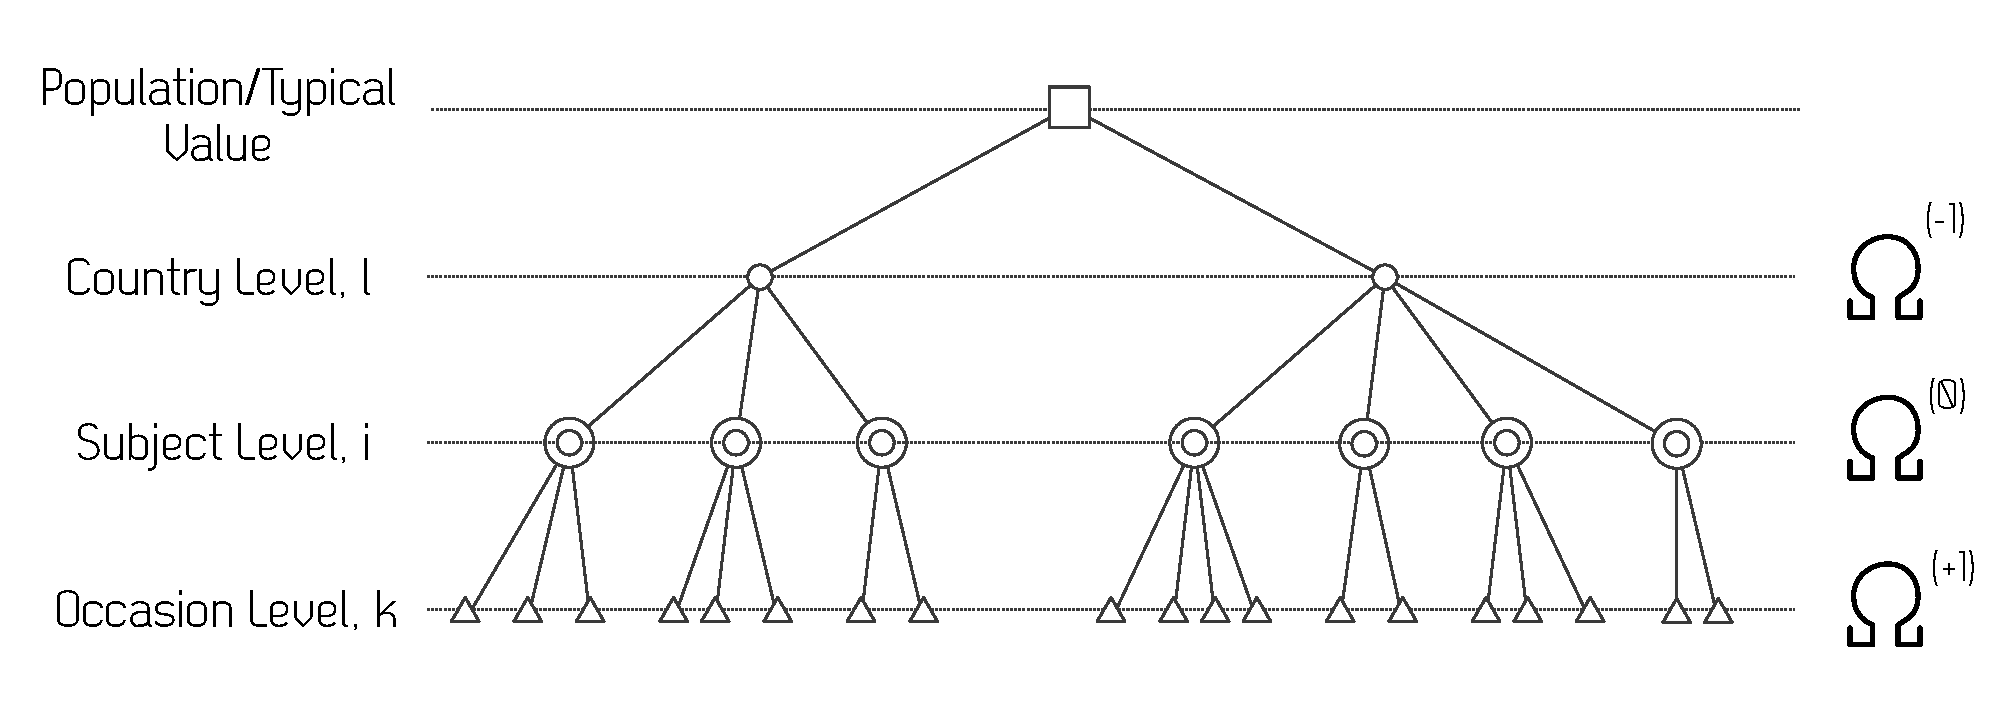
\includegraphics[width=140mm]{pics/HyperVarLevels.pdf}
 \caption{Higher variability levels.}
 \label{fig:interCountry}
\end{figure}

The following code snippet illustrates the implementation in PharmML of 
this complex variability model
\lstset{language=XML}
\begin{lstlisting}
        <VariabilityModel blkId="vm1" type="parameterVariability">
            <Level symbId="country"/>
            <Level referenceLevel="true" symbId="indiv">
                <ParentLevel>
                    <ct:SymbRef symbIdRef="country"/>
                </ParentLevel>
            </Level>
            <Level symbId="iov">
                <ParentLevel>
                    <ct:SymbRef symbIdRef="indiv"/>
                </ParentLevel>
            </Level>
        </VariabilityModel>
\end{lstlisting}

'Country' covariate is stored, when using the explicit design, in \xelem{IndividualCovariates} tag.
The dataset definition and mappings read

\lstset{language=XML}
\begin{lstlisting}
        <Covariates>
            <IndividualCovariates>
                <ColumnMapping>
                    <ds:ColumnRef columnIdRef="COUNTRY"/>
                    <ct:SymbRef blkIdRef="cm1" symbIdRef="Country"/>
                </ColumnMapping>
                <ColumnMapping>
                    <ds:ColumnRef columnIdRef="COUNTRY"/>
                    <ct:SymbRef blkIdRef="vm1" symbIdRef="country"/> 
                </ColumnMapping>
                <!-- ... -->
                <ds:DataSet>
                    <ds:Definition>
                        <ds:Column columnId="ID" columnType="id" valueType="string" columnNum="1"/>
                        <ds:Column columnId="ARM" columnType="arm" valueType="string" columnNum="2"/>
                        <!-- ... -->
                        <ds:Column columnId="COUNTRY" columnType="covariate varLevel" valueType="string" columnNum="5"/>
                    </ds:Definition>
                    <ds:Table>
\end{lstlisting}

As before the \emph{varLevel} value allows to indicate the double use of 
column \xatt{COUNTRY} and the need to map it accordingly to a level 
of the variability model.


%%%%%%%%%%%%%%%%%%%%%%%%%%%%%%%%%%%%%%%%%%%%%%%%%%%%%%%%%%%%%%%%
\section{Changed in the schema}
\label{sec:schemaChanges}
%%%%%%%%%%%%%%%%%%%%%%%%%%%%%%
\subsection{Attribute \xatt{symbolType} for variables is optional}
Now, instead of providing the mandatory attribute e.g.
\lstset{language=XML}
\begin{lstlisting}
			<ct:Variable symbId="CONC" symbolType="real">
\end{lstlisting}
it can be skipped and simply encoded as 
\lstset{language=XML}
\begin{lstlisting}
			<ct:Variable symbId="CONC">
\end{lstlisting}
The same applies to \xelem{DerivativeVariable}.


%%%%%%%%%%%%%%%%%%%%%%%%%%%%%%
\subsection{Integer declaration unification}

The following data types\footnote{All definition are provided on \url{http://www.w3schools.com/xml/schema_dtypes_numeric.asp}}
\begin{itemize}
\item 
\xatt{integer} -- an integer value
\item 
\xatt{positiveInteger} -- an integer containing only positive values (1,2,..)
\end{itemize}
are replaced by
\begin{itemize}
\item 
\xatt{int} -- signed 32-bit integer
\end{itemize}
The positivity validation on certain elements where this is desired, and were
previously encoded using \xatt{positiveInteger}, will be performed in the libPharmML API.

%%%%%%%%%%%%%%%%%%%%%%%%%%%%%%
\subsection{Piecewise namespace correction}
It was pointed out that the \xelem{Piecewise} element occurs in more 
than one namespace. This was due to using the related type, for example 
\lstset{language=XML}
\begin{lstlisting}
                    <xs:element name="Piecewise" type="math:PiecewiseType"/>
\end{lstlisting}
instead of a reference
\lstset{language=XML}
\begin{lstlisting}
                    <xs:element ref="math:Piecewise"/>
\end{lstlisting}
This redundancy has been now removed and the piecewise statement is consistently
declared across all PharmML schemas. 

\smallskip
For some of use cases it means that those using this element have to be corrected.
For example in one of the Product 4.1 use examples instead of
\lstset{language=XML}
\begin{lstlisting}
			<design:ColumnMapping>
				<ds:ColumnRef columnIdRef="AMT"/>
				<ds:Piecewise>
					<math:Piece>
						<ct:SymbRef blkIdRef="sm" symbIdRef="GUT"/>
						<math:Condition>
							<math:LogicBinop op="gt">
								<ds:ColumnRef columnIdRef="AMT"/>
								<ct:Int>0</ct:Int>
							</math:LogicBinop>
						</math:Condition>
					</math:Piece>
				</ds:Piecewise>
			</design:ColumnMapping>
\end{lstlisting}
the namespace prefix has to be changed from \xatt{ds} to \xatt{math} i.e. 
\lstset{language=XML}
\begin{lstlisting}
			<design:ColumnMapping>
				<ds:ColumnRef columnIdRef="AMT"/>
				<math:Piecewise>
					<math:Piece>
						<ct:SymbRef blkIdRef="sm" symbIdRef="GUT"/>
						<math:Condition>
							<math:LogicBinop op="gt">
								<ds:ColumnRef columnIdRef="AMT"/>
								<ct:Int>0</ct:Int>
							</math:LogicBinop>
						</math:Condition>
					</math:Piece>
				</math:Piecewise>
			</design:ColumnMapping>

\end{lstlisting}
In general, this change should not impact any of the converters using the libPharmML.



%%%%%%%%%%%%%%%%%%%%%%%%%%%%%%%%%%%%%%%%%%%%%%%%%%%%%%%%%%%%%%%%
\section{ODEs in conditionals}
\label{sec:ODEinCS}

Ordinary differential equations are from now on allowed in \xelem{ConditionalStatement} 
which means an extension of the rules defined in section \ref{subset:rulesCS}.
As with variables and parameters, the \xelem{DerivativeVariable} has to be 
first declared at the root level of \xelem{StructuralModel} using the attribute \xatt{symbId} 
and then it can be assigned in the conditional statement if required using \xatt{symbIdRef}
as the following example shows

\lstset{language=XML}
\begin{lstlisting}
            <ct:DerivativeVariable symbId="Q1"/>
            <ct:DerivativeVariable symbId="Q2"/>

            <ConditionalStatement>
                <math:If>
                    <math:Condition>
                        <math:LogicBinop op="lt">
                            <ct:SymbRef symbIdRef="t"/>
                            <ct:SymbRef symbIdRef="tmax1"/>
                        </math:LogicBinop>
                    </math:Condition>
                    <ct:DerivativeVariable symbIdRef="Q1">
                        <ct:Assign>
                            <!-- omitted RHS -->
                        </ct:Assign>
                    </ct:DerivativeVariable>
                    <ct:DerivativeVariable symbIdRef="Q2">
                        <ct:Assign>
                            <!-- omitted RHS -->
                        </ct:Assign>
                    </ct:DerivativeVariable>
                </math:If>
                <math:ElseIf>
                    <math:Condition>
                        <math:LogicBinop op="geq">
                            <ct:SymbRef symbIdRef="t"/>
                            <ct:SymbRef symbIdRef="tmax1"/>
                        </math:LogicBinop>
                    </math:Condition>
                    <ct:DerivativeVariable symbIdRef="Q1">
                        <ct:Assign>
                            <!-- omitted RHS -->
                        </ct:Assign>
                    </ct:DerivativeVariable>
                    <ct:DerivativeVariable symbIdRef="Q2">
                        <ct:Assign>
                            <!-- omitted RHS -->
                        </ct:Assign>
                    </ct:DerivativeVariable>
                </math:ElseIf>
                <math:Else>
                    <!-- something else -->
                </math:Else>
            </ConditionalStatement>
\end{lstlisting}


%%%%%%%%%%%%%%%%%%%%%%%%%%%%%%%%%%%%%%%%%%%%%%%%%%%%%%%%%%%%%%%%
\section{Minor changes}
\label{sec:minors}

\begin{itemize}
\item
\xatt{gamma} function has been introduced
\item
Encoding of standard normal distribution -- it is a suggested change in the 
encoding practise. Its implementation became very easy with ProbOnto. Instead 
of the encoding $N(0,1)$ via the Normal1 parameterisation with the lengthily code
\lstset{language=XML}
\begin{lstlisting}
                <RandomVariable symbId="epsilon_Css">
                    <ct:VariabilityReference>
                        <ct:SymbRef blkIdRef="vm2" symbIdRef="resErr"/>
                    </ct:VariabilityReference>
                    <Distribution>
                        <po:ProbOnto name="Normal1">
                            <po:Parameter name="mean">
                                <ct:Assign>
                                    <ct:Real>0</ct:Real>
                                </ct:Assign>
                            </po:Parameter>
                            <po:Parameter name="stdev">
                                <ct:Assign>
                                    <ct:Real>1</ct:Real>
                                </ct:Assign>
                            </po:Parameter>
                        </po:ProbOnto>
                    </Distribution>
                </RandomVariable>
\end{lstlisting}
it is simply enough to declare the available standard normal distribution with code 
name \xatt{StandardNormal1} as following snippet shows
\lstset{language=XML}
\begin{lstlisting}
               <RandomVariable symbId="epsilon_Css">
                    <ct:VariabilityReference>
                        <ct:SymbRef blkIdRef="vm2" symbIdRef="resErr"/>
                    </ct:VariabilityReference>
                    <Distribution>
                        <po:ProbOnto name="StandardNormal1"/>
                    </Distribution>
                </RandomVariable>
\end{lstlisting}
\end{itemize}

